\section{讲解笔记：【第7次作业笔记】 拱结构(1)}
\begin{analysisbox}
本节按题目、答案和讲解笔记顺序整理。对扫描图中的结构几何关系，正文保留 OCR 可识别文字，并在图形页中保留清理后的题图，便于核对杆件、支座、荷载和尺寸。
\end{analysisbox}
\subsection*{第 1 页转写}
结力基础班第7次作业  拱结构

三铰拱作业及答案

I

i

圝礼

Mk

0

Mkt57 F 70 2 0

Mk二年kmu

IMA二01 12 13

48 10

o 6 3 0

 可13 70KN

I ME0

48 4

1 4区B

6  0

 Fx13 57KN

y

4器

1  刈二tx

ii.gl 

f 10 i

i

m

C

A

B 去B 45KN

45kW

TFy

IMA 0

12郦

20 了一zox6 0

打13 15KN

IMc

0

2FxB

6F413 0

扒了45KN
\begin{figure}[H]\centering
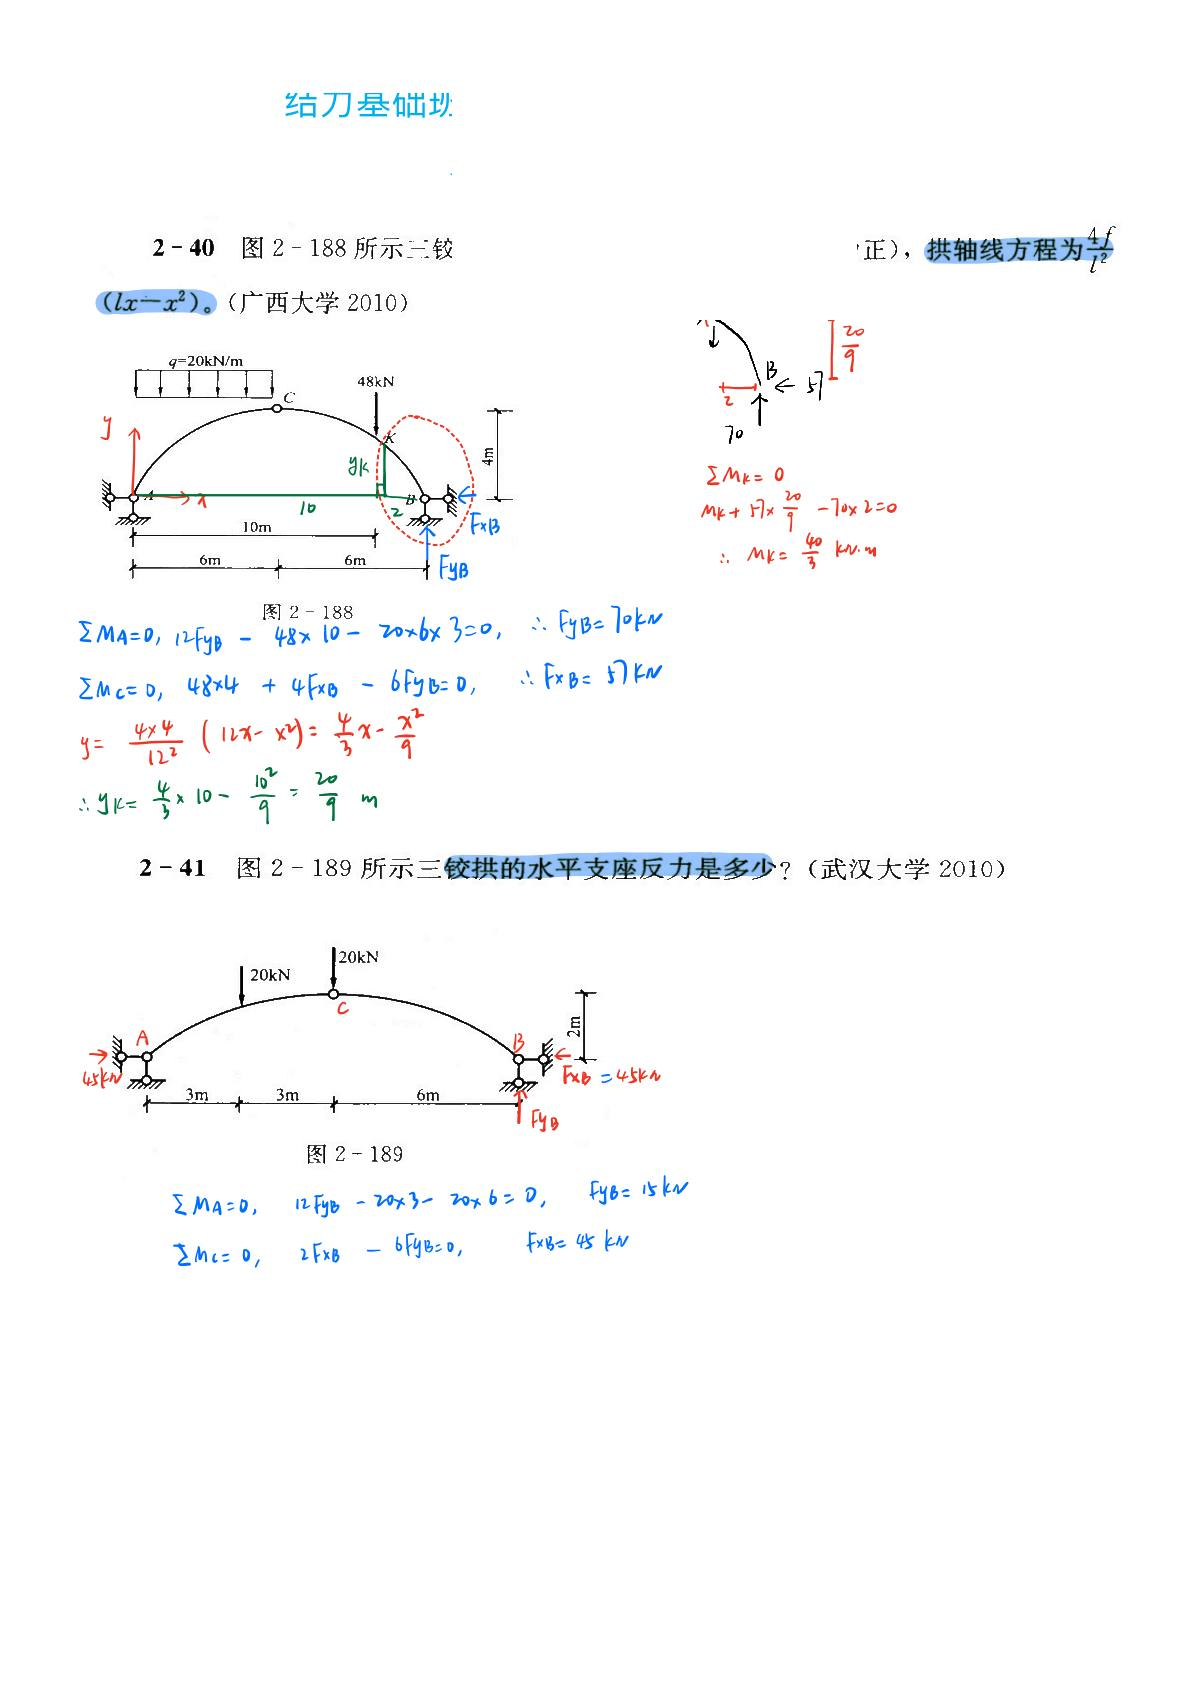
\includegraphics[width=0.92\textwidth]{figures/src27_p001.jpg}
\caption{【第7次作业笔记】 拱结构(1) 第 1 页清理图形页}
\end{figure}
\subsection*{第 2 页转写}
二 

cfo



\_\_

Ty

Ti

EMc 0

FNABX   X 二0

FyDxl

h i

o

i yRip

i FNA13

印

491外侧受拉

zmy

nnnnnnnfn

16FyB 9x8x4ii.ly13 29

M

0

f

B

4在13

29 8 0

二区13 49

xnmii.iq

g

4昔必以12

127

3 nimfjnIm

y

4岩

16x\_x2

x ii

y

1  1 f

yi

1 Y

I

1

i

M 

49

sin0  

达 Fnnx 49 F 六0

w  

可

点噐 

笙

以4

49 F 六一告知49 o

Fsno
\begin{figure}[H]\centering
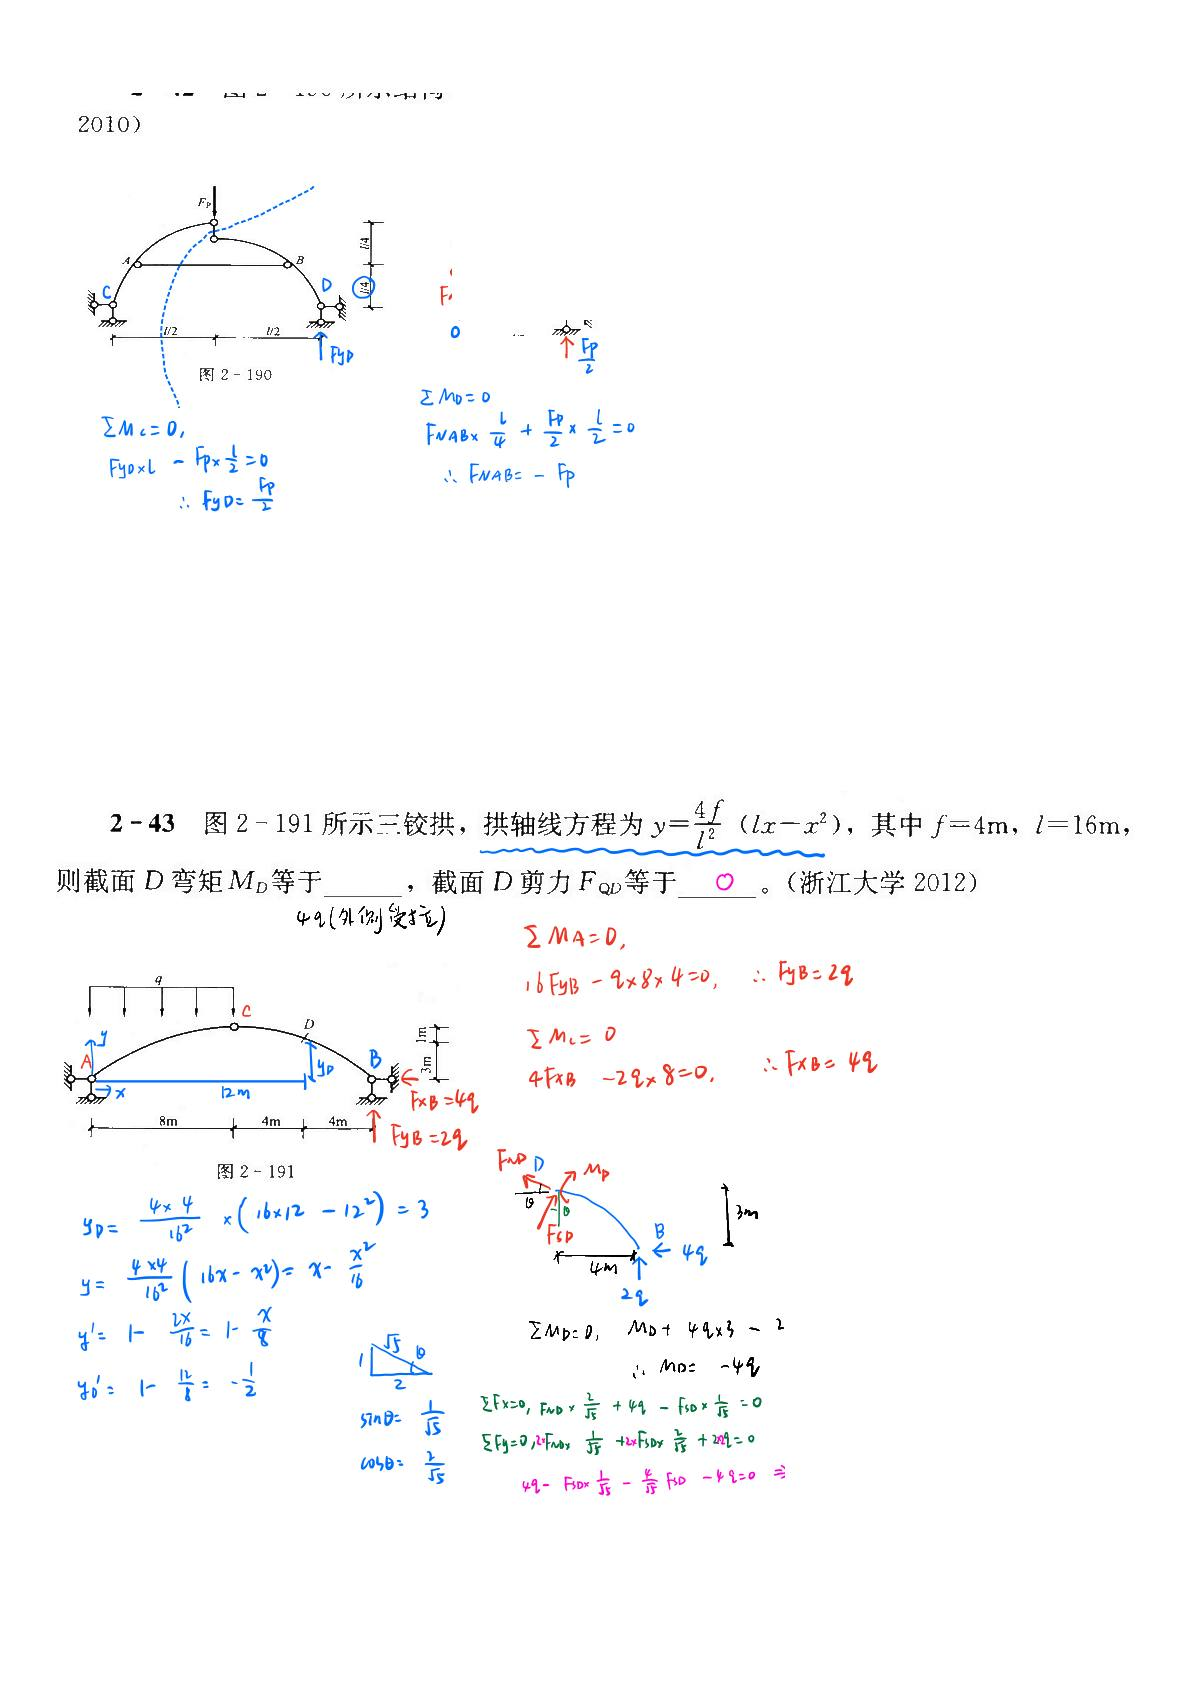
\includegraphics[width=0.92\textwidth]{figures/src27_p002.jpg}
\caption{【第7次作业笔记】 拱结构(1) 第 2 页清理图形页}
\end{figure}
